
\documentclass[ms.tex]{subfiles}
\begin{document}

\section{Nucleosynthesis}
\label{sec:yields}

In this paper we make use of the chemical evolution model for the Milky Way
presented in~\citet{Johnson2021}.
This model runs using the publicly available~\texttt{Versatile Integrator for
Chemical Evolution} (\vice;~\citealp{Johnson2020, Griffith2021, Johnson2021}),
an open-source~\python~package designed for GCE modeling.
\citet{Johnson2021} focus their discussion of the model predictions on O and
Fe, and we retain their yields of these elements here.
As required by~\vice, the SN yields are defined as the net mass of some element
X produced over all explosion events in units of the progenitor cluster's
mass.
For example, with a yield of~$y_\text{X} = 0.001$, a hypothetical~$1000 M_\odot$
star cluster would produce~$1 M_\odot$ of the element X instantaneously in the
case of core collapse supernovae (CCSNe) or over the delay-time distribution
(DTD) in the case of SNe Ia.
We adopt the following values from~\citet{Johnson2021}, who in turn base them
off of~\citet*{Weinberg2017} and~\citet{Johnson2020}:
\begin{itemize}
	\item $y_\text{O}^\text{CC}$ = 0.015

	\item $y_\text{Fe}^\text{CC}$ = 0.0012

	\item $y_\text{O}^\text{Ia}$ = 0

	\item $y_\text{Fe}^\text{Ia}$ = 0.00214
\end{itemize}
We also assume that N is not produced in significant amounts by SNe Ia
\citep{Johnson2019}, and set~$y_\text{N}^\text{Ia}$ throughout this paper
accordingly.
We spend the remainder of this section detailing our CCSN and AGB star yields
of N.

\subsection{Core Collapse Supernovae and Massive Star Winds}
\label{sec:yields:ccsne}

In~\vice, CCSN nucleosynthetic products are approximated to be produced
instantaneously following an episode of star formation; this is a valid
approximation due to how short the lives of massive stars are compared to the
relevant timescales for GCE.
Based on this and its definition as being in units of a stellar population's
total mass, the yield is simply the constant of proportionality between the
CCSN production rate and the star formation rate (SFR):
\begin{equation}
\dot{M}_\text{X}^\text{CC} = y_\text{X}^\text{CC}\dot{M}_\star
\end{equation}
More generally,~$y_\text{X}^\text{CC}$ quantifies~\textit{all} of the
nucleosynthetic material approximated to be produced instantaneously following
a single stellar population's formation, though the majority of such events
for which this approximation is valid will be associated with massive stars
and/or their supernovae.
In the case of N specifically, a substantial amount emerges in winds before the
actual supernova itself, allowing massive stars to produce a lot N even if they
collapse directly to a black hole~\citep{Griffith2021}.

\begin{figure*}
\centering
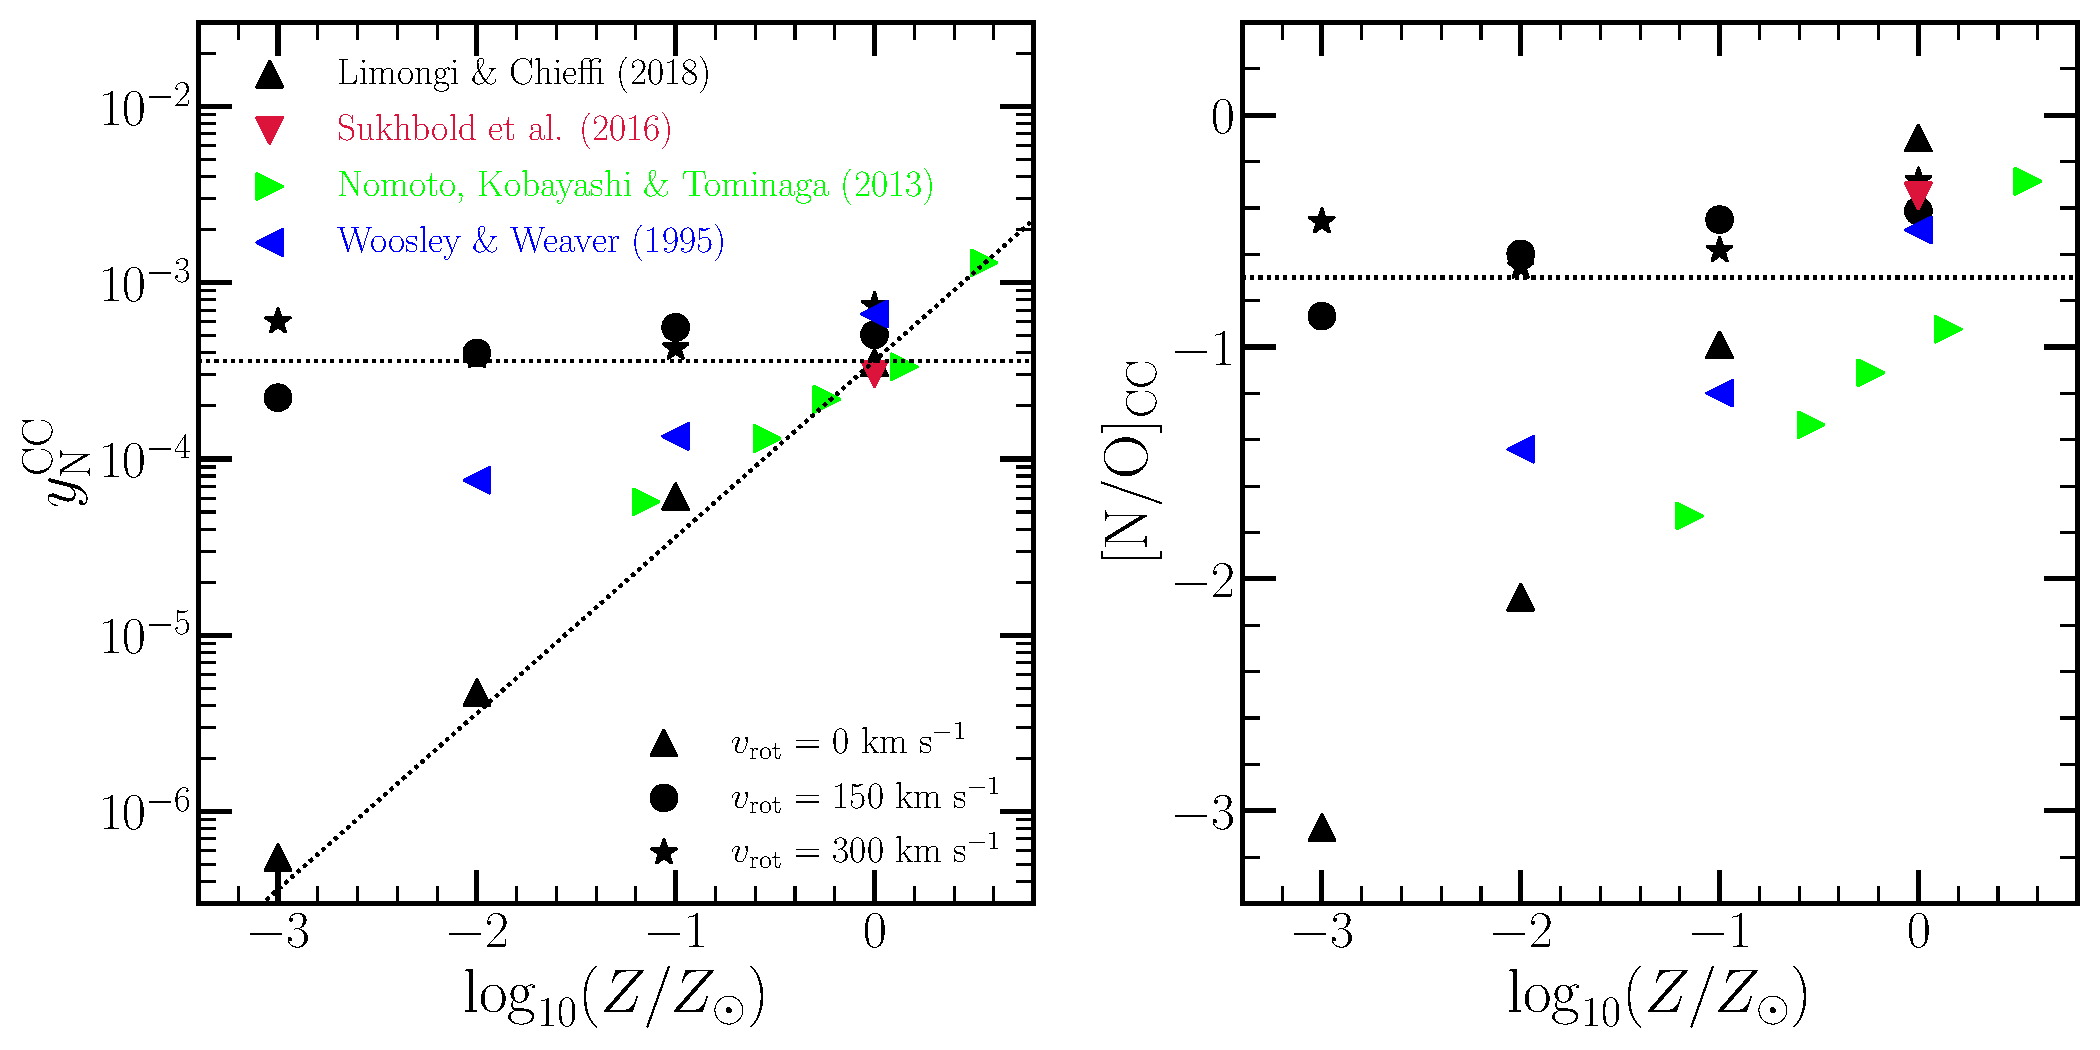
\includegraphics[scale = 0.45]{n_cc_yields.pdf}
\caption{
\textbf{Left}: IMF-averaged CCSN yields of N calculated using~\vice's
\texttt{vice.yields.ccsne.fractional} function with the tables published by
\citet[][blue]{Woosley1995},~\citet[][green]{Nomoto2013},
\citet[][red]{Sukhbold2016}, and~\citet[][black]{Limongi2018}.
All studies report yields for non-rotating progenitors, shown by the triangles;
for visual clarity, the triangles point in a different direction for each study
according to the legend.
\citet{Limongi2018} report additional yields for progenitors with rotational
velocities of 150 (circles) and 300 km/s (stars).
The horizontal dashed line markes~$y_\text{N}^\text{CC} = 3.6\times10^{-4}$,
the value of our fiducial CCSN yield of N in our GCE models.
We use the form shown by the slanted line (equation X) in~\S~X in combination
with some of our AGB star yield models discussed in~\S~\ref{sec:yields:agb}.
\textbf{Right}: The [N/O] ratio predicted by each of the explosion models in
the left-hand panel, under the same colour-coding and marker scheme.
We mark the position of [N/O] = $-0.7$ with a black dotted line, the value
roughly suggested by the observations of low-metallicity systems highlighted
in Fig.~\ref{fig:no_oh_observed}.
}
\label{fig:n_cc_yields}
\end{figure*}

We compute theoretically predicted values of~$y_\text{N}^\text{CC}$ using
\vice's~\texttt{vice.yields.ccsne.fractional} function assuming a
\citet{Kroupa2001} IMF; details on how~\vice~handles these calculations can be
found in~\S~4 of~\citet{Griffith2021} and in the~\vice~science 
documentation\footnote{
\url{https://vice-astro.readthedocs.io/en/latest/science_documentation/yields}
}.
In the left panel of Fig.~\ref{fig:n_cc_yields}, we plot the results as a
function of progenitor metallicity as predicted by the~\citet{Woosley1995},
\citet*{Nomoto2013},~\citet{Sukhbold2016}, and~\citet{Limongi2018} tables.
There is good agreement between the various non-rotating models, but only
\citet{Limongi2018} report yields for progenitors with non-zero rotational
velocities; these yields are substantially larger than that of their
non-rotating counterparts.
Most of the N production in CCSN progenitors occurs via the CNO cycle
processing C and O isotopes into~\Nfourteen, and with few C and O seed nuclei
at low~$Z$, production of~\Nfourteen~is difficult.
Rotation-induced mixing, a highly uncertain process~\citep{Zahn1992, Maeder1998,
Lagarde2012}, could transport newly produced C and O into the hydrogen burning
shell of the CCSN progenitor, facilitating~\Nfourteen~production
(\citealp{Frischknecht2016}; see also discussion in~\S~4.2 of
\citealp{Andrews2017}).
For this reason, N yields at low metallicity are quite sensitive to these
assumptions about stellar rotation and internal mixing processes
\citep{Heger2010}, and consequently IMF-averaged yields are highly uncertain.
\par
Based on the definition of the abundance ratio [X/Y], we can compute the [N/O]
ratio of CCSN ejecta from the values of~$y_\text{N}^\text{CC}$
and~$y_\text{O}^\text{CC}$ predicted from a given yield table:
\begin{equation}
\text{[N/O]}\subcc = 
\log_{10}\left(\frac{y_\text{N}^\text{CC}}{y_\text{O}^\text{CC}}\right) -
\log_{10}\left(\frac{Z_{\text{N},\odot}}{Z_{\text{O},\odot}}\right),
\label{eq:no_subcc}
\end{equation}
where~$Z_{\text{X},\odot}$ is the abundance by mass of some element X in the
sun, for which we take~$Z_{\text{N},\odot} = 6.91\times10^{-4}$ and
$Z_{\text{O},\odot} = 5.72\times10^{-3}$ based on the solar photospheric
abundances of~\citet{Asplund2009}.
For each of the published yield tables and rotational velocities in the left
panel of Fig.~\ref{fig:n_cc_yields}, we compute the corresponding values of
$y_\text{O}^\text{CC}$ using~\vice and plot the resultant values of 
[N/O]\subcc~in the right panel.
These yield ratios follow similar trends with progenitor metallicity and
rotation as~$y_\text{N}^\text{CC}$ itself, a consequence of the fact that these
studies predict relatively metallicity-independent O yields.
\par
CCSN yields can to some extent be empirically calibrated by ensuring that they
reproduce the [N/O] ratios of low metallicity systems.
Since AGB star yields of N are believed to depend on the progenitor's
metallicity (see discussion in~\S~\ref{sec:yields:agb} and references therein),
it's likely that the ``plateau'' in [N/O] at low [O/H] reflects the
IMF-averaged CCSN yields of N and O.
Fig.~\ref{fig:no_oh_observed} suggests that [N/O]\subcc~=~$-0.7$; we highlight
this value in the right panel of Fig.~\ref{fig:n_cc_yields} with a horizontal
black dashed line.
Given this observational result and our adopted value of~$y_\text{O}^\text{CC}$
= 0.015, we compute that an empirical N yield of
$y_\text{N}^\text{CC} = 3.6\times10^{-4}$ using equation~\refp{eq:no_subcc}.
We adopt this value as our fiducial CCSN yield of N and highlight it with a
horizontal black dashed line in the left panel of Fig.~\ref{fig:n_cc_yields}.
We discuss the sloped dotted line in that panel in the context of some of our
AGB star yield models in~\S~X.
\par
These empirical values of [N/O]\subcc~and~$y_\text{N}^\text{CC}$ are in good
agreement with the rotating CCSN models of~\citet{Limongi2018}.
This supports the recent argument by~\citet{Grisoni2021} that rotating massive
stars play an important role in establishing the N abundances observed at low
metallicities in the Milky Way.
Although the~\citet{Sukhbold2016} tables agree nearly perfectly with our
empirical value of~$y_\text{N}^\text{CC} = 3.6\times10^{-4}$, they overestimate
[N/O]\subcc~by~$\sim$0.2 dex; this is because they predict a value of
$y_\text{O}^\text{CC}$ lower than our adopted value of 0.015.
Although most of the supernova models plotted in Fig.~\ref{fig:n_cc_yields}
slightly overestimate our empirical value of [N/O]\subcc~=~$-0.7$, they still
fall short of solar.
This implies the need for an additional enrichment, which is expected because
it is well understood that N is also produced in considerable amounts by
AGB stars~\citep{Johnson2019}.


\subsection{Asymptotic Giant Branch Stars}
\label{sec:yields:agb}

\subsection{IMF-Averaged AGB Star Yields: Metallicity and Time Dependence}
\label{sec:yields:imf_agb}


\end{document}
